% ~~~~~~~~~~~~ %
% tab size = 4 %
% ~~~~~~~~~~~~ %

% WARNING: if the compiler returns the error ``incompatible list can't be unboxed''
% try to decomment the following \RequirePackage command:
%\RequirePackage{atbegshi} 

\documentclass % ~~~~~~~~~~~~~~~~~~~~~~~~~~~~~~~~~~~~~~~~~~~~~~~~~~ %
[																	%
	aspectratio=1610,                                               %
	11pt,															%
	hyperref={pdfpagelabels=false},									%
	xcolor	= pdftex, dvipsnames, table,							%
% 	handout,														% decomment for handouts
]																	%
{beamer}															%
%																	%
\usepackage[latin1]{inputenc}										%
\usepackage[english]{babel}											%
\usepackage{type1cm}												%
\usepackage{type1ec}												%
\usepackage[T1]{fontenc}											%
\usepackage{lmodern}												%
\usepackage{amsmath, amssymb, amsfonts, amsthm}						%
\usepackage{graphicx}												%
\usepackage{hyperref}												%
\usepackage{booktabs}												%
\usepackage{bm}														%
\usepackage{tikz}		                                            %
                                                                    %
\setbeamerfont{note page}{size=\large}                              %
%                                                                   %
% \usetikzlibrary{arrows,decorations.text,decorations.pathmorphing}	%
% \usetikzlibrary{decorations.footprints,fadings,calc,trees,mindmap}%
% \usetikzlibrary{shadows,patterns,positioning,shapes,matrix,fit}	%
% \usetikzlibrary{intersections,datavisualization,plotmarks,spy}	%
\usepackage{pgfplots}												%
% \pgfplotsset{compat=1.3}											%
%\usetikzlibrary{external}											%
%\tikzexternalize[shell escape=-enable-write18]						%
%																	%
\usepackage{pgfpages}												%
\setbeamercovered{invisible}
\setbeameroption{show notes on second screen=left}					% comment for just 1 screen
%																	%
% ~~~~~~~~~~~~~~~~~~~~~~~~~~~~~~~~~~~~~~~~~~~~~~~~~~~~~~~~~~~~~~~~~ %
%																	%
\def\DarkBlue		{black!70!blue}%{black!40!blue}					%
\def\DarkGray		{black!70!white}								%
\def\DarkGreen		{black!40!green}								%
\def\DarkRed		{black!40!red}									%
\def\DarkYellow		{black!40!yellow}								%
\def\DarkOrange		{black!40!orange}								%
%																	%
\def\Blue			{black!30!blue}									%
\def\Gray			{black!50!white}								%
\def\Green			{black!10!green}								%
\def\Red			{black!10!red}									%
\def\Yellow			{black!10!yellow}								%
\def\Orange			{black!10!orange}								%
%																	%
\def\LightBlue		{white!40!blue}									%
\def\LightGray		{white!92!black}%{white!70!white}				%
\def\LightGreen		{white!40!green}%{white!40!green}				%
\def\LightRed		{white!40!red}									%
\def\LightYellow	{white!40!yellow}								%
\def\LightOrange	{white!40!orange}								%
%																	%
% ~~~~~~~~~~~~~~~~~~~~~~~~~~~~~~~~~~~~~~~~~~~~~~~~~~~~~~~~~~~~~~~~~ %
%																	%
\def\Background		{white}%{\pgfsetfillopacity{.95}}%{white}		%
\def\Foreground		{\DarkBlue}%{black}								%
\def\Primary		{\Blue}%{\Blue}									%
\def\Secondary		{\LightGray}%{\Gray}							%
%																	%
\def\StrongPrimary	{\Primary!80!black}								%
\def\SoftPrimary	{\Primary!20!white}								%
\def\StrongSecondary{\Secondary!80!black}							%
\def\SoftSecondary	{\Secondary!20!white}							%
%																	%
% ~~~~~~~~~~~~~~~~~~~~~~~~~~~~~~~~~~~~~~~~~~~~~~~~~~~~~~~~~~~~~~~~~ %
%																	%
\graphicspath{{./Images/}}											%
%																	%
\input{Scripts/newcommands}											%
\input{Scripts/theme}												%
%																	%
% ~~~~~~~~~~~~~~~~~~~~~~~~~~~~~~~~~~~~~~~~~~~~~~~~~~~~~~~~~~~~~~~~~ %
%																	%
%\title		[Short title]		{Sensor integration for high\\      %
%                                temperature measurements}			%
\title		[Short title]		{Sensor Integration for High\\      %
                                Temperature Measurements}			%                                
\date		{May 31, 2017} % empty = no dates. Alternatives: {\today} / {April 20, 2099}
\institute	[Short institute]	{Lule\r{a} University of Technology\\
    Dept. of Computer Science, Electrical and Space Engineering \\
    Div. of EISLAB}							                        %
\author		[Short author]		{David Ragnarsson}					%
%																	%
\begin{document}													%
%																	%
% ~~~~~~~~~~~~~~~~~~~~~~~~~~~~~~~~~~~~~~~~~~~~~~~~~~~~~~~~~~~~~~~~~ %

\usebackgroundtemplate{\includegraphics[width=\paperwidth, height=\paperheight]{Images/background_eng.jpg}}
%\addtobeamertemplate{block begin}{\pgfsetfillopacity{0.9}}{\pgfsetfillopacity{.9}}
% title page
\begin{frame}
	%
	\titlepage
	%
	\begin{center}
		\includegraphics[height = 1.5cm]{Images/L_dekor_en.png}
		\qquad
		\includegraphics[height = 1.5cm]{Images/disire_logo.png}
	\end{center}
	
	\note{ put your notes here }
	%
\end{frame}


% table of contents 
\section*{Table of contents}
\begin{frame}
	%
	\frametitle{Table of Contents}
	\tableofcontents[subsectionstyle=hide]	% [show | shaded | hide]
	
	\note{ This is the structure of the presentation }
	%
\end{frame}


\section{Introduction}

\begin{frame}
	%
	\frametitle{Table of Contents}
	\tableofcontents[subsectionstyle=hide,
	                currentsection]	% [show | shaded | hide]
	
	\note{ Start with some introduction and background to the problem }
	%
\end{frame}

\begin{frame}
	%
	\frametitle{Mining Industry Today}
	\framesubtitle{Introduction}
	
	\begin{itemize}
		%
		\visible<1->{\item{Expensive equipment}}
		\visible<2->{\item{Stationary measurements}}
		\visible<3->{\item{Temperature, Oxygen \& Humidity}}
		\visible<4->{\item{Optimized industry process}}
		%
	\end{itemize}
	
	
	\note{ High temperature measurements are expensive and not well integrated with the material.
	
	        Why is this a problem?
	        
	        Why oxygen specific?
	        
	        Temperature, oxygen, humidity are of interest.
	        
	        Optimized process saves money and energy}
	%
\end{frame}

\begin{frame}
    %
    \frametitle{Previous Work}
    \framesubtitle{Introduction}
    
    \begin{itemize}
        \visible<1->{\item{Wireless measurements in high temperatures}}
        \visible<2->{\item{Temperature measurements}}
        \visible<3->{\item{Oxygen sensor selected}}
    \end{itemize}
    
    \note{ Wireless measurement with radio frequency
    
            Temperature wireless in oven
            
            Suggested and tested oxygen sensor in this type of environment}
    %
\end{frame}



\begin{frame}
	%
	\frametitle{Oxygen Sensor}
	\framesubtitle{Introduction}
	%
	\begin{block}{Bosch LSU4.9 - benefits}
		%
		\begin{itemize}
		%
		\visible<1->{\item{Operates in high temperatures}}
		\visible<2->{\item{Tested in these environments}}
		\visible<3->{\item{Independent of reference gas}}
		%
	\end{itemize}
		%
	\end{block}
	
	%
	\vspace{0.6cm}
	%
	
	\visible<4->{
	\begin{block}{Bosch LSU4.9 - drawbacks}
		%
		\begin{itemize}
		%
		\item<4->{Reacts to multiple substances}
		\item<5->{Temperature dependent}
		\item<6->{Size}
		%
	\end{itemize}
		%
	\end{block}}
	
	
	\note{ compensatinos have to be made due to temperature and other substance if they are reactable
	
	        Size can be a problem when the system has to be smaller }
	%
\end{frame}


\begin{frame}
	%
	\frametitle{System Overview}
	\framesubtitle{Introduction}
	%
	\begin{itemize}
		%
		\visible<1->{\item{Control unit communicates with Radio unit}}
		\visible<2->{\item{Data is sent wireless to antennas mounted inside the oven}}
		%
	\end{itemize}
	
	%
	\vspace{0.8cm}
	%
	
	\begin{figure}
	    \centering
	    \includegraphics[width=\textwidth]{Images/systemoverview_trans.png}
	\end{figure}
	
	\note{ Control unit is the electronics circuit built in this thesis
	
	        I2C standard digital communication protocol}
	%
\end{frame}

%%%%%%%%%%%%%%%%%%%%%%%%%%%%%%%%%%%%%%%%%%%%%%%%%%%%%
%                       Method                      %
%%%%%%%%%%%%%%%%%%%%%%%%%%%%%%%%%%%%%%%%%%%%%%%%%%%%%
\section{Method}

\begin{frame}
	%
	\frametitle{Table of Contents}
	\tableofcontents[subsectionstyle=hide,
	                currentsection]	% [show | shaded | hide]
	
	\note{ put your notes here }
	%
\end{frame}


\begin{frame}
	%
	\frametitle{Lab Bench}
	\framesubtitle{Method}
	%    
	
	\begin{columns}[c] % [ b | c | t | T | onlytextwidth | totalwidth ]
		\begin{column}{0.5\textwidth}
			\begin{center}
			    \includegraphics[width=\textwidth]{Images/lambda_bench.png}
			\end{center}
		\end{column}
%		%
%		% -----------------------------------------------
		\begin{column}{0.5\textwidth}
			\begin{itemize}
			    \visible<1->{\item Power supply for heating up sensor}
			    \visible<2->{\item Vise to avoid heating damages}
			    \visible<3->{\item 20.95 \% O$_2$ in air}
			\end{itemize}
		\end{column}	
    \end{columns}
    
    \note{ In real test no power supply is available
    
            oxygen level is also lower}
    %
\end{frame}


\begin{frame}
	%
	\frametitle{Bosch LSU4.9 Electrical Equivalent}
	\framesubtitle{Method}
	%    
	
	\begin{columns}[c] % [ b | c | t | T | onlytextwidth | totalwidth ]
		\begin{column}{0.5\textwidth}
			\begin{center}
			    \includegraphics[width=\textwidth]{Images/SCHEMATIC1_lsu49_trans.png}
			\end{center}
		\end{column}
%		%
%		% -----------------------------------------------
		\begin{column}{0.5\textwidth}
			\begin{itemize}
			    \visible<1->{\item 4 of 6 connectors used}
			    \visible<2->{\item Rcal sensor specific}
			    \visible<3->{\item Nernst cell oxygen dependent}
			    \visible<4->{\item Nernst resistance temperature dependent}
			\end{itemize}
		\end{column}	
    \end{columns}
    
    \note{ Rcal is replaced by surface mounted resistor
    
            Ip and oxygen level can change the nernst cell voltage
            
            AC signal used to calculate the nernst resistance and also the temperature}
    %
\end{frame}



\begin{frame}
	%
	\frametitle{Prototyping on Breadboard}
	\framesubtitle{Method}
	%    
	
	\begin{columns}[c] % [ b | c | t | T | onlytextwidth | totalwidth ]
		\begin{column}{0.5\textwidth}
			\begin{center}
			    \includegraphics[width=\textwidth]{Images/breadboard.png}
			\end{center}
			\vspace{1cm}
		\end{column}
%		%
%		% -----------------------------------------------
		\begin{column}{0.5\textwidth}
			\begin{itemize}
			    \visible<1->{\item DIL package \& IC-adapters}
			    \visible<2->{\item Verify simulations}
			    \visible<3->{\item Easy to change components}
			    \visible<4->{\item Instead of using development board}
			\end{itemize}
			\vspace{1cm}
		\end{column}	
    \end{columns}
    
    \note{ PIC with DIL package
    
            Different resistor and capacitors can be tested with ease
            
            This replace the use of development board}
    %
\end{frame}



\begin{frame}
	%
	\frametitle{Schematic for MCU}
	\framesubtitle{Method}
	%    
	
	\begin{columns}[c] % [ b | c | t | T | onlytextwidth | totalwidth ]
		\begin{column}{0.65\textwidth}
			\begin{center}
			    \includegraphics[width=\textwidth]{Images/PIC18_schematic.png}
			\end{center}
		\end{column}
%		%
%		% -----------------------------------------------
		\begin{column}{0.35\textwidth}
			\begin{itemize}
    			\visible<1->{\item PIC18F26K22}
			    \visible<2->{\item Two I$^2$C buses}
			    \visible<3->{\item USART for debugging}
			    \visible<4->{\item PWM for temperature}
			    \visible<5->{\item 5 ADC measurements}
			\end{itemize}
		\end{column}	
    \end{columns}
    
    \note{ I2C to Radio and DAC
    
            USART to bluetooth circuit
            
            PWM is the AC signal
            
            The ADC measurements used to calculate oxygen level and temperature}
    %
\end{frame}


\begin{frame}
	%
	\frametitle{PCB Layout}
	\framesubtitle{Method}
	%    
	
	\begin{columns}[c] % [ b | c | t | T | onlytextwidth | totalwidth ]
		\begin{column}{0.75\textwidth}
			\begin{center}
			    \includegraphics[width=\textwidth]{Images/PCB_layout.png}
			\end{center}
		\end{column}
%		%
%		% -----------------------------------------------
		\begin{column}{0.25\textwidth}
			\begin{itemize}
			    \visible<1->{\item Digital \& analog GND/Supply}
			    %\visible<2->{\item Two supply planes}
			    \visible<2->{\item 4 layers}
			\end{itemize}
		\end{column}	
    \end{columns}
    
    \note{ Bigger connectors on supply and programming connectors for simplicity \\
            LSU 4.9 connector too small \\
            Separate ground planes \\
            4 layer gives better possibility to place components on two sides}
    %
\end{frame}


\begin{frame}
	%
	\frametitle{Mounted PCB}
	\framesubtitle{Method}
	%    
	
	\begin{columns}[c] % [ b | c | t | T | onlytextwidth | totalwidth ]
		\begin{column}{0.65\textwidth}
			\begin{center}
			    \includegraphics[width=\textwidth]{Images/PCB_monterad.png}
			\end{center}
		\end{column}
%		%
%		% -----------------------------------------------
		\begin{column}{0.35\textwidth}
			\begin{itemize}
			    \visible<1->{\item Patches with wire}
			    %\visible<2->{\item Empty positions}
			    %\visible<3->{\item PWM for temperature}
			    %\visible<4->{\item 4 ADC measurements}
			\end{itemize}
		\end{column}	
    \end{columns}
    
    \note{ Patches to set different level on reference pin
    
            Empty spots for optional components}
    %
\end{frame}


\begin{frame}
	%
	\frametitle{Software}
	\framesubtitle{Method}
	%    
	
	\begin{columns}[c] % [ b | c | t | T | onlytextwidth | totalwidth ]
		\begin{column}{0.65\textwidth}
			\begin{center}
			    \includegraphics[width=\textwidth]{Images/Software_map_trans.png}
			\end{center}
		\end{column}
%		%
%		% -----------------------------------------------
		\begin{column}{0.35\textwidth}
			\begin{itemize}
			    \visible<1->{\item Clock speed 16 MHz}
			    \visible<2->{\item I$^2$C slave to radio unit}
			    %\visible<3->{\item PWM in 2 kHz}
			    %\visible<4->{\item 4 ADC measurements}
			\end{itemize}
		\end{column}	
    \end{columns}
    
    \note{ First initialize functions and pins, like I2C och PWM \\
            Stays in control loop for 3 seconds before entering sleep}
    %
\end{frame}



\begin{frame}
	%
	\frametitle{Electronics Before Waterproofing}
	\framesubtitle{Method}
	%    
	
	\begin{columns}[c] % [ b | c | t | T | onlytextwidth | totalwidth ]
		\begin{column}{0.65\textwidth}
			\begin{center}
			    \includegraphics[width=\textwidth]{Images/electronics_box.png}
			\end{center}
		\end{column}
%		%
%		% -----------------------------------------------
		\begin{column}{0.35\textwidth}
			\begin{itemize}
			    \visible<1->{\item Antenna \& sensors goes outside}
			    \visible<2->{\item Communication wires between PCBs}
			    \visible<3->{\item Box keeps silicon in place}
			    %\visible<4->{\item 4 ADC measurements}
			\end{itemize}
			\vspace{2cm}
		\end{column}	
    \end{columns}
    
    \note{ Antenna temperature oxygen goes outside
    
            Box is filled with silicon for water proofing}
    %
\end{frame}



\begin{frame}
	%
	\frametitle{Final Mechanical Construction}
	\framesubtitle{Method}
	%    
	
	\begin{columns}[c] % [ b | c | t | T | onlytextwidth | totalwidth ]
		\begin{column}{0.5\textwidth}
			\begin{center}
			    \includegraphics[height = 6.5cm]{Images/mechanical_construction_cropped.png}
			\end{center}
		\end{column}
%		%
%		% -----------------------------------------------
		\begin{column}{0.5\textwidth}
			\begin{center}
			    \includegraphics[height = 6.5cm]{Images/water_box.png}
			\end{center}
		\end{column}	
    \end{columns}
    
    \note{ Box to right is filled with water and flower foam
    
            Electronics inside black box and flipped into the box with water}
    %
\end{frame}



%%%%%%%%%%%%%%%%%%%%%%%%%%%%%%%%%%%%%%%%%%%%%%%%%%%%%
%                       Results                     %
%%%%%%%%%%%%%%%%%%%%%%%%%%%%%%%%%%%%%%%%%%%%%%%%%%%%%
\section{Results}

\begin{frame}
	%
	\frametitle{Table of Contents}
	\tableofcontents[subsectionstyle=hide,
	                currentsection]	% [show | shaded | hide]
	
	\note{ put your notes here }
	%
\end{frame}



\begin{frame}
	%
	\frametitle{Measurements During First Test at Mefos}
	\framesubtitle{Results}
	%
	\begin{itemize}
		%
		\visible<1->{\item{Passes from zone 1 to 3}}
		\visible<2->{\item{Averaging from LSU4.9 measurement}}
		%
	\end{itemize}
	
	%
	\vspace{0.3cm}
	%
	
	\begin{figure}
	    \centering
	    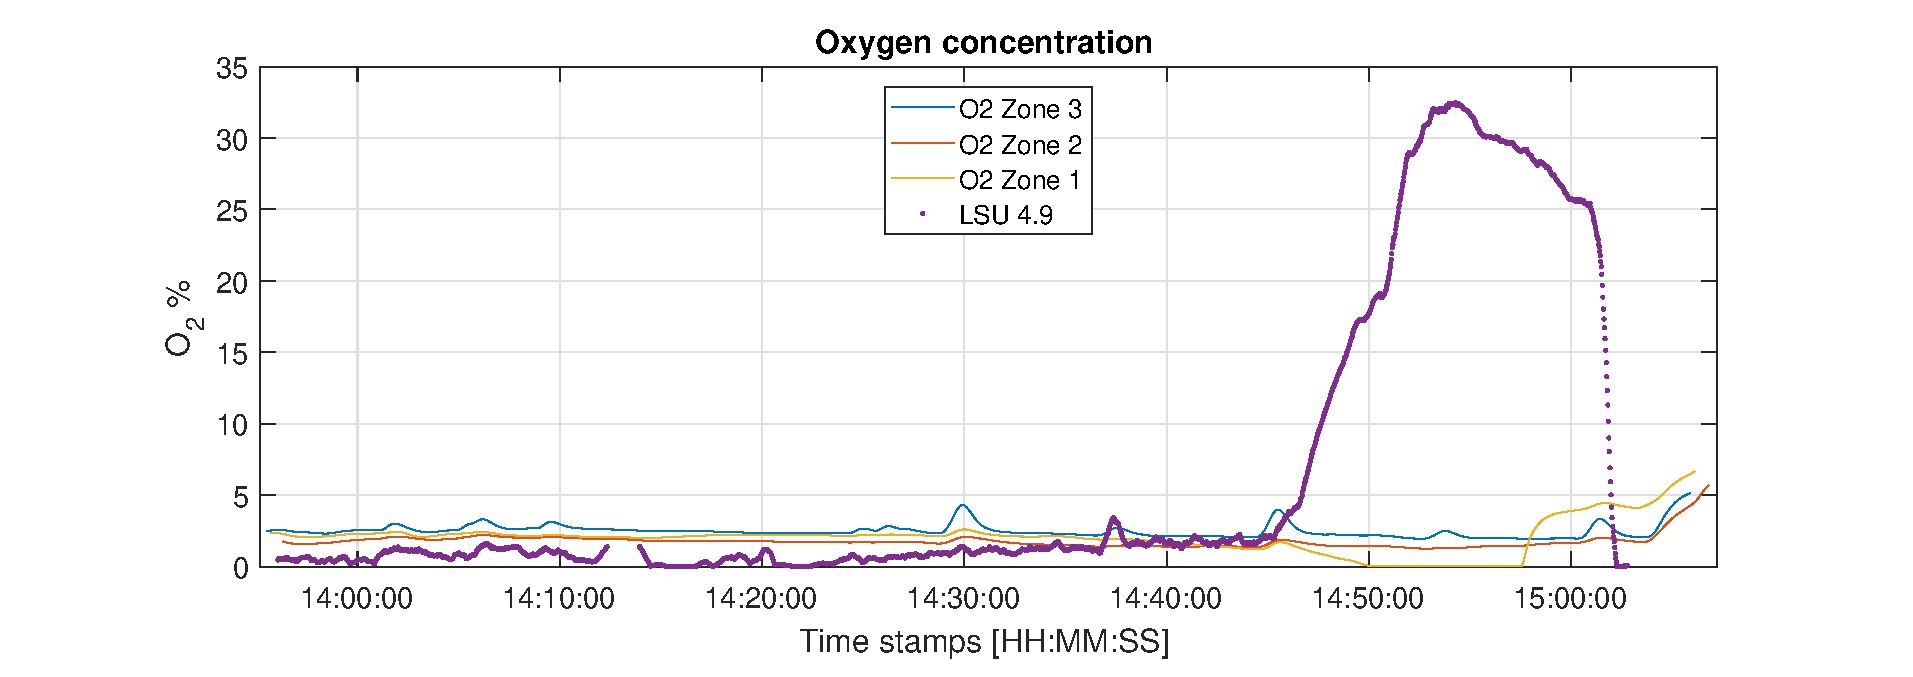
\includegraphics[width=\textwidth]{Images/syre_dots_trans.eps}
	\end{figure}
	
	\note{ Same time in the different zones
	
	        The oxygen values are averaging
	        
	        No good explanation for the peak at the end}
	%
\end{frame}



\begin{frame}
	%
	\frametitle{Measurements from a Small Oven at Mefos}
	\framesubtitle{Results}
	%
	\begin{itemize}
		%
		\visible<1->{\item{Raw values}}
		\visible<2->{\item{Compensated for temperature differences}}
		%
	\end{itemize}
	
	%
	\vspace{0.3cm}
	%
	
	\begin{figure}
	    \centering
	    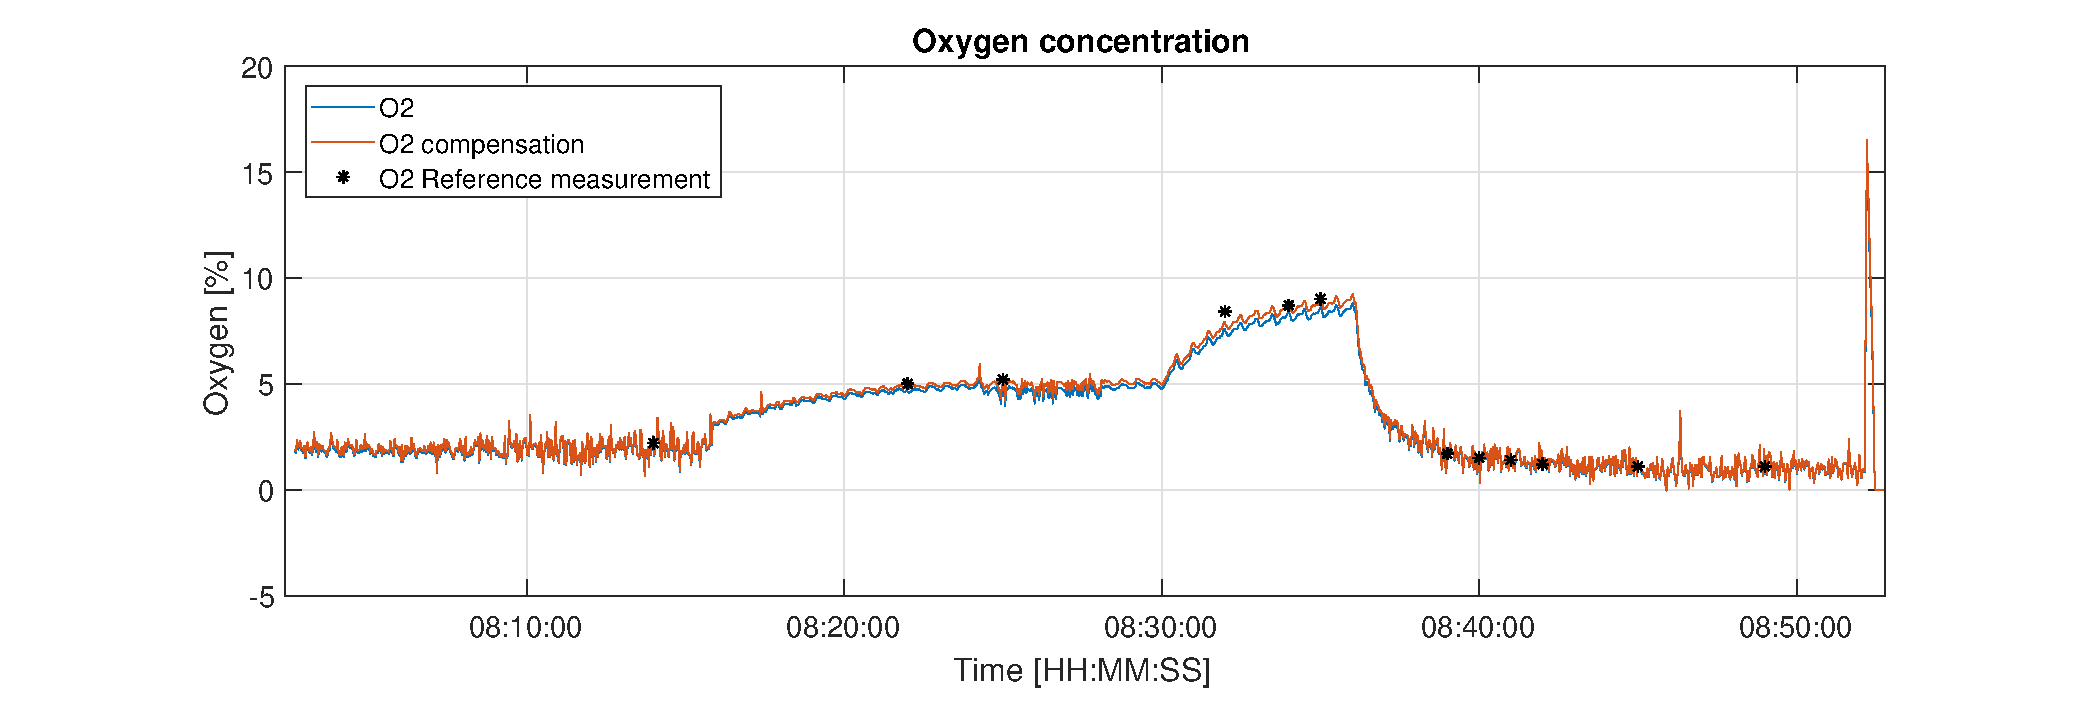
\includegraphics[width=\textwidth]{Images/oxygen_second_small_trans.eps}
	\end{figure}
	
	\note{ Done in a small oven at Mefos
	
	        Reliable values
	        
	        Referece values are logged manually}
	%
\end{frame}



%%%%%%%%%%%%%%%%%%%%%%%%%%%%%%%%%%%%%%%%%%%%%%%%%%%%%
%                   Discussion                      %
%%%%%%%%%%%%%%%%%%%%%%%%%%%%%%%%%%%%%%%%%%%%%%%%%%%%%
\section{Discussion}

\begin{frame}
	%
	\frametitle{Table of Contents}
	\tableofcontents[subsectionstyle=hide,
	                currentsection]	% [show | shaded | hide]
	
	\note{ put your notes here }
	%
\end{frame}



\begin{frame}
	%
	\frametitle{Conclusion}
	\framesubtitle{Discussion}
	%
	\begin{itemize}
		%
        \visible<1->{\item If higher robustness is achieved, the approach is good}
	    \visible<2->{\item Slow to reach operating temperature in oven}
	    %\visible<3->{\item }
	    %\visible<4->{\item 4 ADC measurements}
		%
	\end{itemize}
	
	\note{ Everything except oxygen sensor works perfect
	
	        Long time to reach correct temperature}
	%
\end{frame}



\begin{frame}
	%
	\frametitle{Future Work}
	\framesubtitle{Discussion}
	%
	\begin{itemize}
		%
        \visible<1->{\item Look into why oxygen values become unreliable after a while in the oven}
	    \visible<2->{\item Run the sensor on one cell battery (3.6 V)}
	    \visible<3->{\item Investigate the possibility to use sensor without housing}
	    %\visible<4->{\item 4 ADC measurements}
		%
	\end{itemize}
	
	\note{ Keep testing the system
	
	        One cell battery gives a smaller size and easier to integrate the system with the radio system
	        
	        The housing is big and massive. It might be good to give a more stable temperature though}
	%
\end{frame}



%\begin{frame}
%	%
%	\frametitle{Frame with two columns}
%	\framesubtitle{(subtitle)}
%	%
%	\begin{columns}[c] % [ b | c | t | T | onlytextwidth | totalwidth ]
%		%
%		% ``columns'' options usage (from the beamer user guide)
%		%
%		% [b] will cause the bottom lines of the columns to be vertically aligned.
%		% [c] will cause the columns to be centered vertically relative to each
%		%     other. Default, unless the global option t is used.
%		% [onlytextwidth] is the same as totalwidth=\textwidth.
%		% [t] will cause the first lines of the columns to be aligned. Default
%		%     if global option t is used.
%		% [T] is similar to the t option, but T aligns the tops of the first lines
%		%     while t aligns the so-called baselines of the first lines. If strange
%		%     things seem to happen in conjunction with the t option (for example
%		%     if a graphic suddenly ``drops down'' with the t option instead of
%		%     ``going up,''), try using this option instead.
%		% [totalwidth= width] will cause the columns to occupy not the whole page
%		%     width, but only width, all told.
%		%
%		% -----------------------------------------------
%		\begin{column}{0.5\textwidth}
%			column one
%		\end{column}
%		%
%		% -----------------------------------------------
%		\begin{column}{0.5\textwidth}
%			column two
%		\end{column}
%		%
%	\end{columns}
%	
%	\note{ put your notes here }
%	%
%\end{frame}





%\begin{frame}
	%%
	%\frametitle{Frame with a movie}
	%\framesubtitle{(subtitle)}
	%%
	%\movie[externalviewer]{text on the slides}{./video.wmw}
	%%
%\end{frame}


% ending page
\section*{}
\begin{frame}
	%
	\titlepage
	%
	\begin{center}
		davrag-2@student.ltu.se \\
		%david.ragnarsson@ltu.se
		%www.ee.kth.se/$\sim$XXXX/
	\end{center}
	
	\note{ put your notes here }
	%
\end{frame}



%%%%%%%%%%%%%%%%%%%%%%%%%%%%%%%%%%%%%%%%%%%%%%%%%%%%%
%                     Appendix                      %
%%%%%%%%%%%%%%%%%%%%%%%%%%%%%%%%%%%%%%%%%%%%%%%%%%%%%
\section*{Appendix}

\begin{frame}

\begin{center}
    \includegraphics[width=.8\textwidth]{Images/Lambdasond_schematic.pdf}
\end{center}
    
\end{frame}


\begin{frame}

\begin{center}
    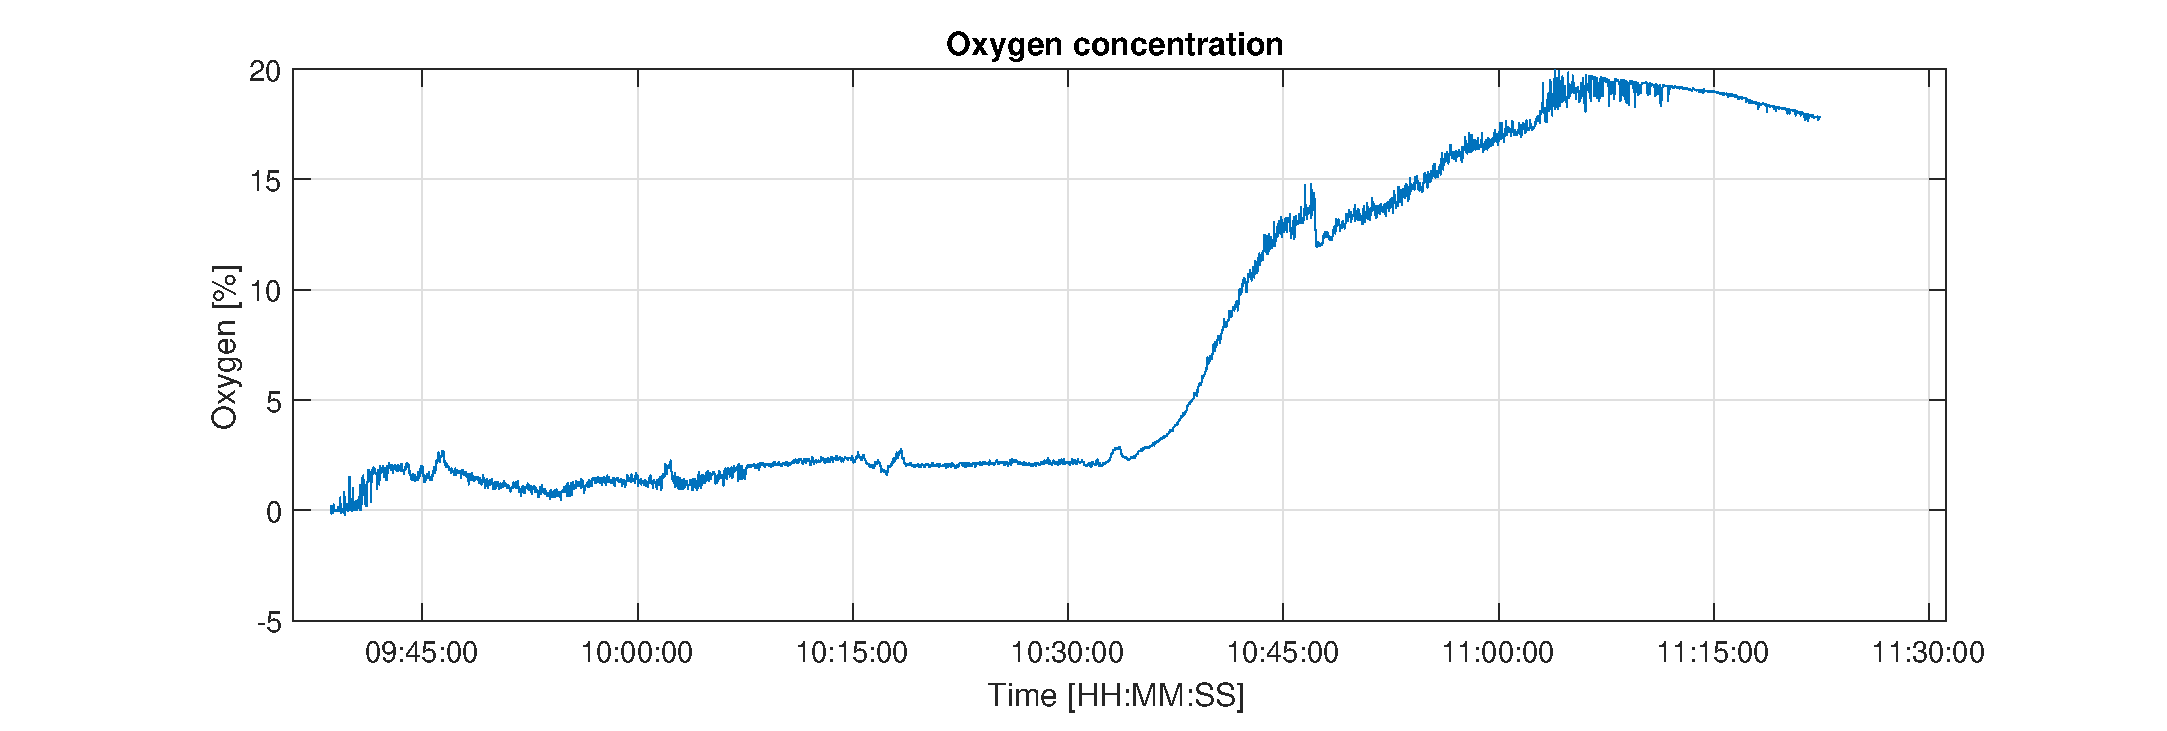
\includegraphics[width=\textwidth]{Images/oxygen_second_big.eps}
\end{center}
    
\end{frame}


\begin{frame}

\begin{center}
    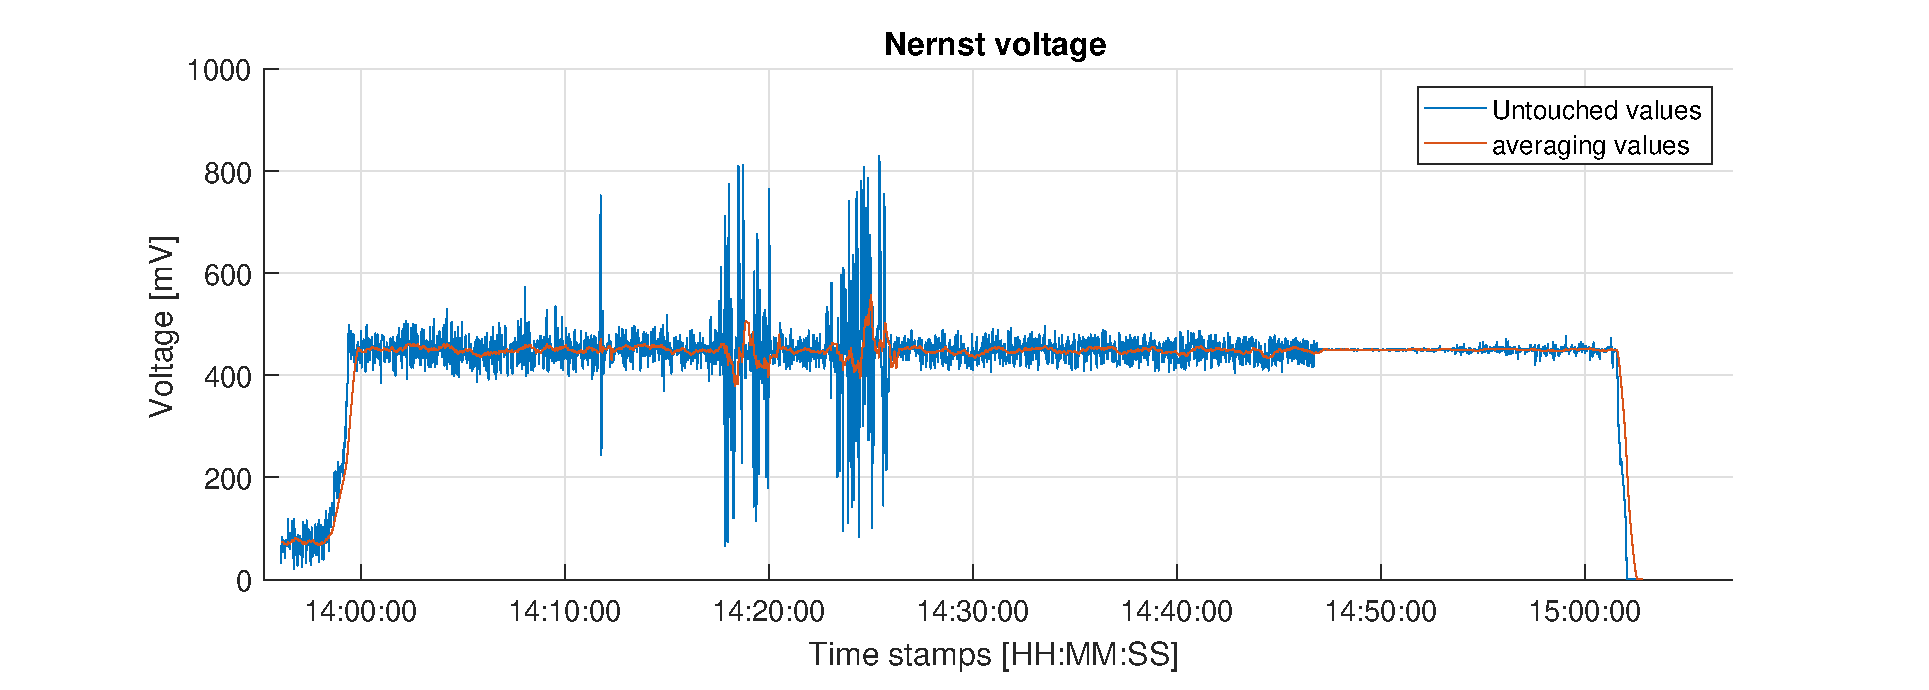
\includegraphics[width=\textwidth]{Images/nernst_both.eps}
\end{center}
    
\end{frame}


\begin{frame}

\begin{center}
    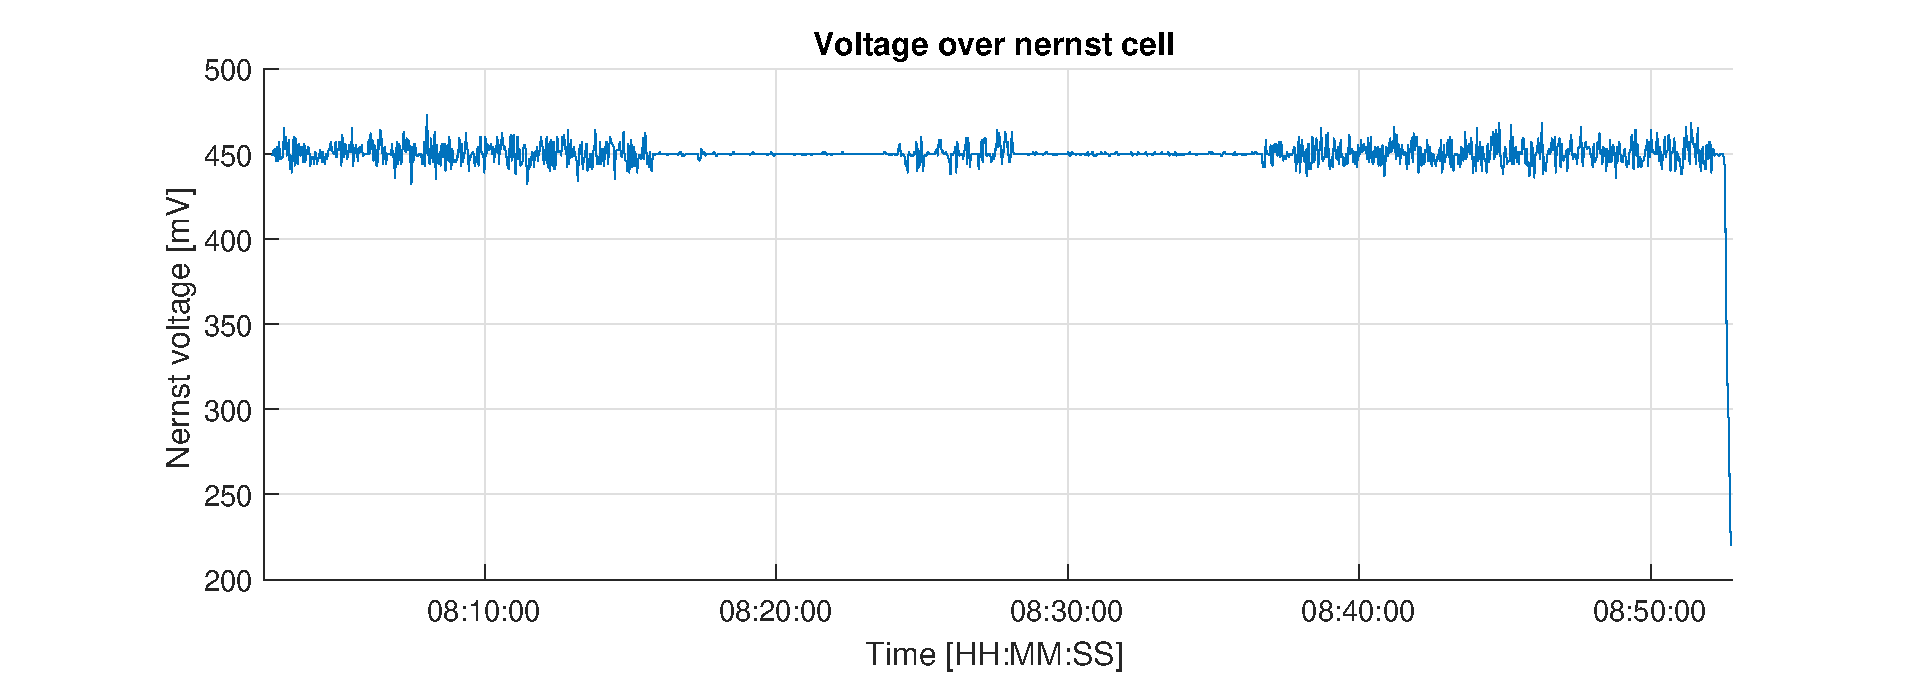
\includegraphics[width=\textwidth]{Images/nernst_second_small.eps}
\end{center}
    
\end{frame}


\begin{frame}

\begin{center}
    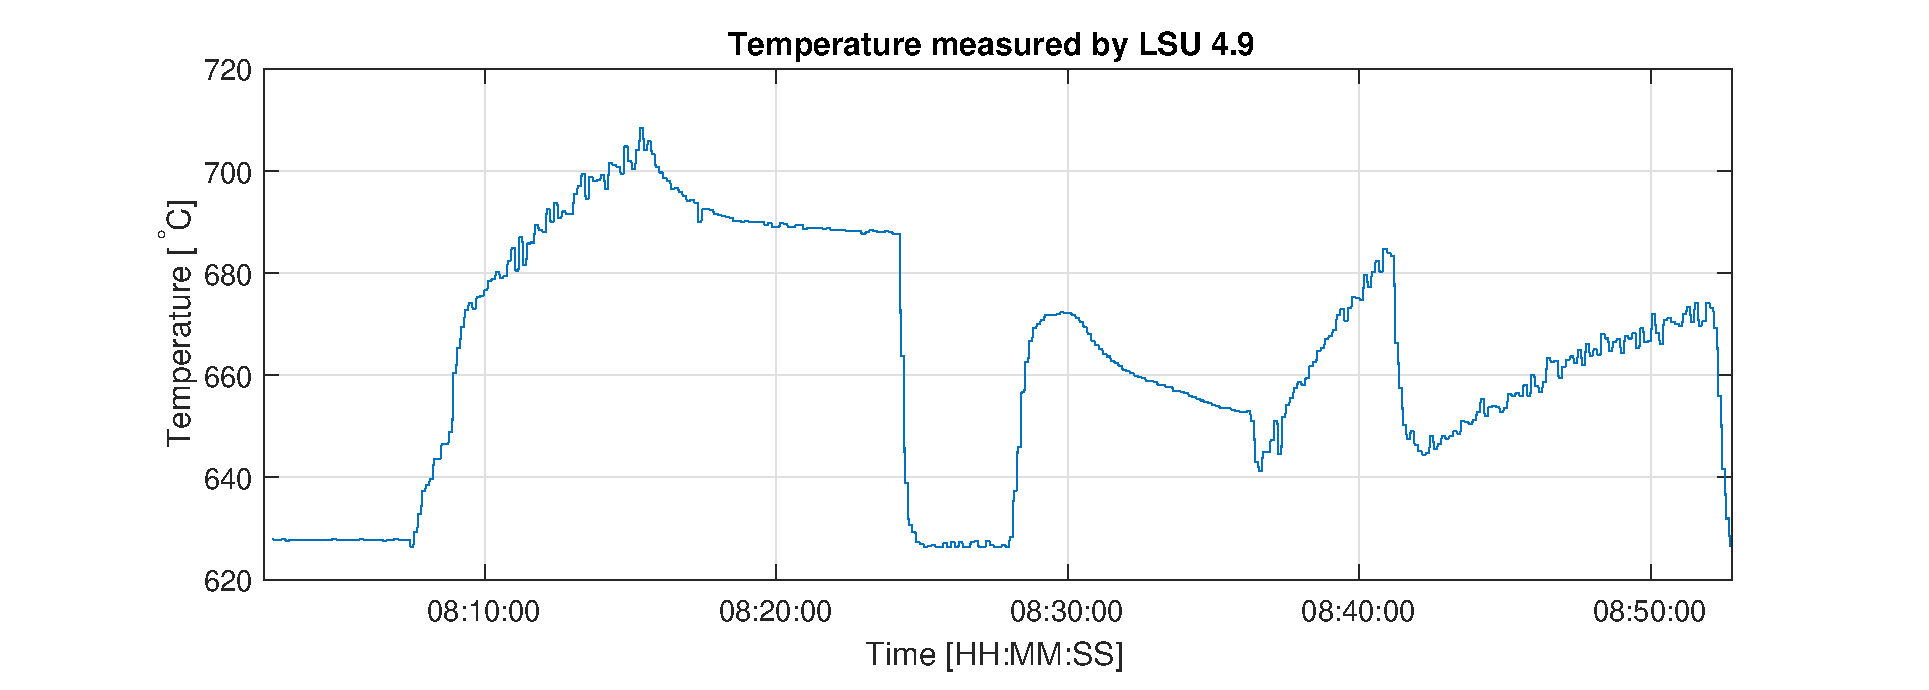
\includegraphics[width=\textwidth]{Images/temperature_second_small.eps}
\end{center}
    
\end{frame}


% bibliography
%\section*{Bibliography}
%\begin{frame}
%\begin{thebibliography}{}
%	%
%	\frametitle{Bibliography}
%	\small
%	%
%	\bibitem[1]{elements_of_style}
%	William Strunk, Jr.\ (1918)
%	\newblock The Elements of Style
%	\newblock Pearson Education Company
%	%
%	\vspace{0.3cm}
%	%
%	\bibitem[2]{promessi_sposi}
%	Alessandro Manzoni (1842)
%	\newblock I promessi sposi
%	\newblock Adelchi
%	
%	\note{ put your notes here }
%	%
%\end{thebibliography}
%\end{frame}


% ~~~~~~~~~~~~~~~~~~~~~~~~~~~~~~~~~~~~~~~~~~~~~~~~~~~~~~~~~~~~~~~~~ %
%																	%
\end{document}														%
%																	%
% ~~~~~~~~~~~~~~~~~~~~~~~~~~~~~~~~~~~~~~~~~~~~~~~~~~~~~~~~~~~~~~~~~ %
